\chapter{Título do segundo capítulo}
\label{cap:fundamentacao-teorica}

    Alguns autores preferem fazer uma "fundamentação teórica" ~no segundo capítulo, outros, preferem fazer uma "revisão da literatura". Entretanto, isto é particular de cada trabalho e o autor deve escolher o título mais adequado. Consultar o orientador é importante para determinar o título apropriado.

    Evite começar da seção secundária, ou seja, não passe direto do título do capítulo para o título da seção secundária. Escreva um texto para introduzir as seções subsequentes. Lembre-se de utilizar primeira letra maiúscula quando estiver se referindo a um objeto com numeração específica como capítulo, seção, subseção, figura, tabela, quadro, equação, normalmente, se escreve a primeira letra maiúscula da palavra do objeto seguido do \textit{label}. Por exemplo, a Seção \ref{sec:citacoes} explica como fazer citações bibliográficas. Observe no código fonte deste texto como foi feita a referência cruzada. Isso permite enumerar a seção do modo automático o que facilita caso novas seções sejam criadas.  

    \section{Citações bibliográficas}
    \label{sec:citacoes}

        Esta frase mostra como citar um livro sobre descargas atmosféricas \cite{rakov2003lightning}. Também podem ser citados sites como \citeonline{elat2015densidade}.

        Referenciando outro site \cite{secretaria1999}. Texto texto texto texto texto texto texto texto texto texto texto texto texto texto texto texto texto texto texto. Texto texto texto texto texto texto texto texto texto texto texto texto texto texto texto texto texto texto texto. Texto texto texto texto texto texto texto texto texto texto texto texto texto texto texto texto texto texto texto. Texto texto texto texto texto texto texto texto texto texto texto texto texto texto texto texto texto texto texto. Citando uma norma \cite{NBR10520:1988}.
        
        Citação de duas referências que concordam entre si \cite{lamport1986latex,Maia2011}. Texto texto texto texto texto texto texto texto texto texto texto texto texto texto texto texto texto texto texto. Texto texto texto texto texto texto texto texto texto texto texto texto texto texto texto texto texto texto texto. Texto texto texto texto texto texto texto texto texto texto texto texto texto texto texto texto texto texto texto. Texto texto texto texto texto texto texto texto texto texto texto texto texto texto texto texto texto texto texto texto texto texto texto texto texto texto. Citando um manual \cite{manuais1989}. 
        
        Outro tipo de citação é a citação literal ou direta com mais de três linhas. Este tipo de citação deve ser destacada com recuo de $4~cm$ da margem esquerda com letra menor (tamanho 10), sem aspas e com espaçamento simples.  Para exemplificar esse tipo de citação, considere a afirmação de \citeonline{feitosa2016}:
        
        \begin{citacao}
            A cultura é o processo através do qual o homem cria o algo onde antes imperava o
            nada. Esse algo é toda complexidade de criações simbólicas, de sentidos e significados que
            damos às coisas e ao mundo. Um “algo” que não se sustenta se não se entender os processos
            culturais como mecanismos de mediação entre nós e os fenômenos. Assim, mais do que
            apenas um elemento da comunicação, a mediação é, por excelência, cultural. As diversas
            modalidades de mediação são apenas sotaques diferenciados dessa mediação cultural. Assim
            é a mediação informacional.
        \end{citacao}
        
        A afirmação do parágrafo anterior também pode ser reproduzida com a citação na final como mostra o exemplo a seguir: 
        
        \begin{citacao}
            A cultura é o processo através do qual o homem cria o algo onde antes imperava o
            nada. Esse algo é toda complexidade de criações simbólicas, de sentidos e significados que
            damos às coisas e ao mundo. Um “algo” que não se sustenta se não se entender os processos
            culturais como mecanismos de mediação entre nós e os fenômenos. Assim, mais do que
            apenas um elemento da comunicação, a mediação é, por excelência, cultural. As diversas
            modalidades de mediação são apenas sotaques diferenciados dessa mediação cultural. Assim
            é a mediação informacional \cite{feitosa2016}.
        \end{citacao}
        
        %Mais exemplos e opções de citações podem ser encontradas em:
        
%        https://en.wikibooks.org/wiki/LaTeX/Bibliography_Management
%        https://github.com/cfgnunes/latex-cefetmg/blob/master/latex-cefetmg/03-elementos-pos-textuais/apendices.tex        
        
        

    \section{Inserindo figuras}
    \label{sec:figuras}
    
    A Figura \ref{fig:reitoria} apresenta a fotografia da reitoria da Universidade Federal do Ceará. Observe a estrutura do código para inserir a Figura \ref{fig:reitoria}. No título, apenas a primeira letra da frase é maiúscula  exceto nomes próprios e não há ponto final. Procure ajustar o tamanho da figura para preencher a largura delimitada pelas margens esquerda e direita. Não esqueça de indicar fonte da figura. 
    
   	\begin{figure}[h!]
		\Caption{\label{fig:reitoria} Fotografia da Reitoria da Universidade Federal do Ceará}
		%\centering
		\UFCfig{}{
			\fbox{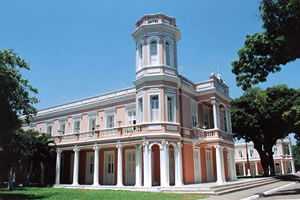
\includegraphics[width=12cm]{figuras/exemplo-1}}
		}{
			\Fonte{\citeonline{UFC2012}.}
		}	
	\end{figure}
	
    Texto texto texto texto texto texto texto texto texto texto texto texto texto texto texto texto texto texto texto texto texto texto texto texto texto texto texto texto texto texto texto texto texto texto texto texto texto texto texto texto texto texto texto texto texto.

    Texto texto texto texto texto texto texto texto texto texto texto texto texto texto texto texto texto texto texto. Texto texto texto texto texto texto texto texto texto texto texto texto texto texto texto texto texto texto texto.

    A Figura \ref{fig:sondas} Texto texto texto texto texto texto texto texto texto texto texto texto texto texto texto texto texto texto texto. Texto texto texto texto texto texto texto texto texto texto texto texto texto texto texto texto texto texto texto.

	\begin{figure}[h!]
		\centering
		\Caption{\label{fig:sondas} Gráfico da Atmosfera Superior}	
		\UFCfig{}{
			\fbox{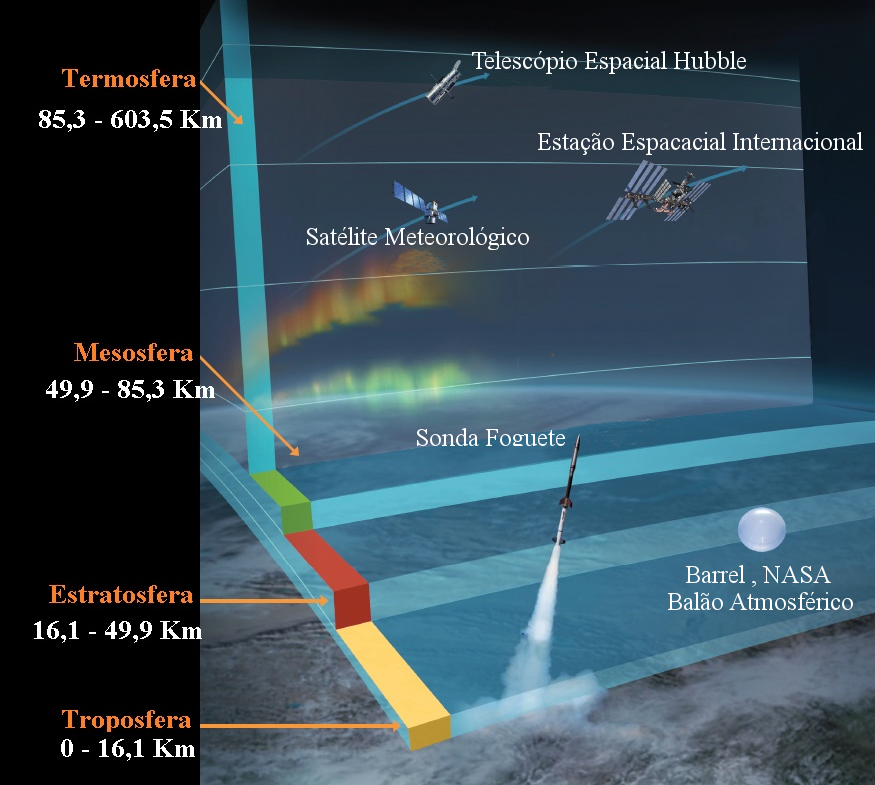
\includegraphics[width=12cm]{figuras/sondas}}
		}{
			\Fonte{adaptado de \citeonline{NASA2016}.}}	
	\end{figure}

    Texto texto texto texto texto texto texto texto texto texto texto texto texto texto texto texto texto texto texto texto texto texto texto texto texto texto texto texto texto texto texto texto texto texto texto texto texto texto texto texto texto texto texto texto texto.

    Texto texto texto texto texto texto texto texto texto texto texto texto texto texto texto texto texto texto texto texto texto texto texto texto texto texto texto texto texto texto texto texto texto texto texto texto texto texto texto texto texto texto texto texto texto.

    Texto texto texto texto texto texto texto texto texto texto texto texto texto texto texto texto texto texto texto texto texto texto texto texto texto texto texto texto texto texto texto texto texto texto texto texto texto texto texto texto texto texto texto texto texto.

    Texto texto texto texto texto texto texto texto texto texto texto texto texto texto texto texto texto texto texto texto texto texto texto texto texto texto texto texto texto texto texto texto texto texto texto texto texto texto texto texto texto texto texto texto texto.

    Texto texto texto texto texto texto texto texto texto texto texto texto texto texto texto texto texto texto texto texto texto texto texto texto texto texto texto texto texto texto texto texto texto texto texto texto texto texto texto texto texto texto texto texto texto.

    \section{Inserindo tabelas}
    \label{sec:tabelas}

	A Tabela \ref{tab:exemplo-1} Texto texto texto texto texto texto texto texto texto texto texto texto texto texto texto texto texto texto texto. Texto texto texto texto texto texto texto texto texto texto texto texto texto texto texto texto texto texto texto.
		
	\begin{table}[h!]	
		\centering
		\Caption{\label{tab:exemplo-1} Exemplo de tabela}	
		\UFCtab{}{
			\begin{tabular}{cll}
				\toprule
				Ranking & Exon Coverage & Splice Site Support \\
				\midrule \midrule
				E1 & Complete coverage by a single transcript & Both splice sites\\
				E2 & Complete coverage by more than a single transcript & Both splice sites\\
				E3 & Partial coverage & Both splice sites\\
				E4 & Partial coverage & One splice site\\
				E5 & Complete or partial coverage & No splice sites\\
				E6 & No coverage & No splice sites\\
				\bottomrule
			\end{tabular}
		}{
		\Fonte{elaborado pelo autor.}
	}
	\end{table}

\subsection{Exemplo de subseção} \label{sec:ex_sec}
	
Texto texto texto texto texto texto texto texto texto texto texto texto texto texto texto texto texto texto texto texto texto texto texto texto texto texto texto texto texto texto texto texto texto texto texto texto texto texto texto texto texto texto texto texto texto.

%acrlong{DATASUS},\acrlong{DNV},\acrlong{DO},\acrlong{ESF},\acrlong{IBGE},\acrlong{MFC},\acrlong{MI},\acrlong{MS},\acrlong{NV},\acrlong{ODM},\acrlong{OI},\acrlong{OMS},\acrlong{ONU},\acrlong{PNI},\acrlong{PSF},\acrlong{RIPSA},\acrlong{RN},\acrlong{SIM},\acrlong{SINASC},\acrlong{SUS},\acrlong{TMI},\acrlong{TMMFC}


\begin{alineascomponto}
	\item Integer non lacinia magna. Aenean tempor lorem tellus, non sodales nisl commodo ut
	\item Proin mattis placerat risus sit amet laoreet. Praesent sapien arcu, maximus ac fringilla efficitur, vulputate faucibus sem. Donec aliquet velit eros, sit amet elementum dolor pharetra eget
	\item Integer eget mattis libero. Praesent ex velit, pulvinar at massa vel, fermentum dictum mauris. Ut feugiat accumsan augue, et ultrices ipsum euismod vitae
	\begin{subalineascomponto}
		\item Integer non lacinia magna. Aenean tempor lorem tellus, non sodales nisl commodo ut
		\item Proin mattis placerat risus sit amet laoreet.
	\end{subalineascomponto}
\end{alineascomponto}

Teste de siglas \gls{TMMFC}, \gls{DA}, \gls{MCEG}